\documentclass[12pt,a4paper]{article}

\usepackage[margin=1in]{geometry}
\usepackage{amsmath, amssymb, amsthm}
\usepackage{enumitem}
\usepackage{booktabs}
\usepackage{tikz}
\usetikzlibrary{arrows.meta, positioning}

\setlength{\parindent}{0pt}
\setlength{\parskip}{6pt}

\newtheoremstyle{notestyle}
  {8pt}
  {8pt}
  {\normalfont}
  {}
  {\bfseries}
  {.}
  {0.5em}
  {}

\theoremstyle{notestyle}
\newtheorem{definition}{Definition}
\newtheorem{example}{Example}
\newtheorem{proposition}{Proposition}

\newenvironment{answer}
{\par\textbf{Answer.}\ }
{\hfill$\square$\par}

\newcommand{\Prob}{\mathbb{P}}
\newcommand{\E}{\mathbb{E}}
\newcommand{\Var}{\operatorname{Var}}

\title{\textbf{Supplementary Notes: Branching Processes, PGFs, Extinction, and Growth}}
\author{MA4034: Time Series and Stochastic Processes}
\date{}

\begin{document}
\maketitle

\section{What is a Branching Process?}

A branching process is a stochastic model for a population that changes generation by generation.

Let
\[
Z_n=\text{number of individuals in generation }n.
\]

Usually,
\[
Z_0=1,
\]
meaning the population starts with one individual.

Each individual produces a random number of children. Let
\[
X=\text{number of children produced by one individual}.
\]

The distribution of $X$ is called the \textbf{offspring distribution}.

\begin{center}
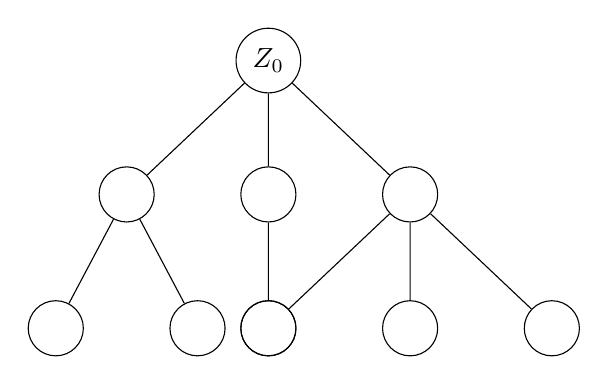
\begin{tikzpicture}[
  person/.style={circle, draw, minimum size=7mm},
  edge/.style={-{Latex[length=2mm]}, thick},
  level distance=17mm,
  sibling distance=18mm
]
\node[person] {$Z_0$}
  child {node[person] {}
    child {node[person] {}}
    child {node[person] {}}
  }
  child {node[person] {}
    child {node[person] {}}
  }
  child {node[person] {}
    child {node[person] {}}
    child {node[person] {}}
    child {node[person] {}}
  };
\end{tikzpicture}
\end{center}

\textbf{Simple analogy.} Think of a family tree. One person has children. Each child then has children. The branching process counts how many people are in each generation.

\section{How is $Z_n$ Calculated?}

Suppose generation $n-1$ has
\[
Z_{n-1}
\]
individuals.

Each of these individuals produces children. Let
\[
X_k=\text{number of children produced by the }k\text{th individual}.
\]

Then the next generation size is
\[
Z_n=\sum_{k=1}^{Z_{n-1}}X_k.
\]

This means:
\[
\text{new population size}=\text{total children produced by current population}.
\]

\begin{example}
Suppose generation 1 has
\[
Z_1=3
\]
individuals. These three individuals produce
\[
2,\quad 0,\quad 4
\]
children respectively. Find $Z_2$.
\end{example}

\begin{answer}
Here,
\[
X_1=2,\qquad X_2=0,\qquad X_3=4.
\]

Therefore,
\[
Z_2=X_1+X_2+X_3.
\]

So
\[
Z_2=2+0+4=6.
\]
\end{answer}

\section{Probability Generating Function}

\begin{definition}[Probability Generating Function]
If $X$ is a non-negative integer-valued random variable, its probability generating function, or PGF, is
\[
G(s)=\E[s^X].
\]
\end{definition}

If
\[
\Prob(X=k)=p_k,
\]
then
\[
G(s)=p_0+p_1s+p_2s^2+p_3s^3+\cdots.
\]

So the PGF stores the probabilities of the offspring distribution.

\[
\begin{array}{c|c}
\text{Term in }G(s) & \text{Meaning}\\
\hline
p_0 & \Prob(X=0)\\
p_1s & \Prob(X=1)\\
p_2s^2 & \Prob(X=2)\\
p_3s^3 & \Prob(X=3)
\end{array}
\]

\textbf{Simple analogy.} The PGF is like a compact code for the offspring distribution. The coefficient of $s^k$ tells you the probability of having $k$ children.

\begin{example}
Suppose
\[
\Prob(X=0)=\frac14,\qquad \Prob(X=2)=\frac34.
\]
Find the PGF.
\end{example}

\begin{answer}
By definition,
\[
G(s)=\E[s^X].
\]

So
\[
G(s)=\frac14s^0+\frac34s^2.
\]

Since
\[
s^0=1,
\]
we get
\[
\boxed{G(s)=\frac14+\frac34s^2.}
\]
\end{answer}

\section{Population Extinction}

Extinction means the population eventually becomes zero.

Let
\[
E=\{\text{event that the population eventually becomes extinct}\}.
\]

If for some generation $n$,
\[
Z_n=0,
\]
then there are no individuals left to reproduce. Therefore,
\[
Z_{n+1}=Z_{n+2}=\cdots=0.
\]

The extinction probability is
\[
\Prob(E).
\]

\section{How PGFs Give Extinction Probability}

Let
\[
q=\Prob(E).
\]

The extinction probability is the smallest solution in $[0,1]$ of
\[
s=G(s).
\]

\begin{proposition}[Extinction Probability]
For a branching process with offspring PGF $G(s)$, the extinction probability $q$ is the smallest solution in $[0,1]$ of
\[
s=G(s).
\]
\end{proposition}

\subsection*{Why Solve $s=G(s)$?}

Suppose one individual has $k$ children.

For the whole population to eventually become extinct, all $k$ children lines must eventually become extinct.

If the extinction probability of one line is $q$, then the probability all $k$ lines die out is
\[
q^k.
\]

Now average over all possible values of $k$:
\[
q=\Prob(X=0)q^0+\Prob(X=1)q^1+\Prob(X=2)q^2+\cdots.
\]

This is exactly
\[
q=G(q).
\]

So we solve
\[
s=G(s).
\]

\section{Population Growth}

The mean number of children per individual is
\[
\mu=\E[X].
\]

This is the most important number for deciding the general behaviour.

\[
\begin{array}{c|c|c}
\text{Case} & \text{Name} & \text{Conclusion}\\
\hline
\mu<1 & \text{subcritical} & \Prob(E)=1\\
\mu=1 & \text{critical} & \Prob(E)=1\\
\mu>1 & \text{supercritical} & \Prob(E)<1
\end{array}
\]

Also,
\[
\E[Z_n]=\mu^n
\]
when
\[
Z_0=1.
\]

\subsection*{Meaning of $\mu$}

If
\[
\mu<1,
\]
then each individual has less than one child on average. The population tends to shrink, and extinction is certain.

If
\[
\mu=1,
\]
then each individual replaces itself on average. This still leads to extinction with probability 1, although extinction may take a long time.

If
\[
\mu>1,
\]
then each individual has more than one child on average. The population has a positive chance of surviving forever.

\section{Can We Conclude Extinction Just from $\mu$?}

Yes and no.

\subsection*{What $\mu$ Can Tell Us}

The value of $\mu$ tells us whether extinction is certain or not.

\[
\boxed{
\mu\leq 1 \quad\Longrightarrow\quad \Prob(E)=1.
}
\]

So if
\[
\mu\leq1,
\]
we can conclude extinction happens with probability 1 without solving for $q$.

Also,
\[
\boxed{
\mu>1 \quad\Longrightarrow\quad \Prob(E)<1.
}
\]

So if
\[
\mu>1,
\]
we can conclude extinction is not certain.

\subsection*{What $\mu$ Cannot Tell Us}

If
\[
\mu>1,
\]
then we only know
\[
\Prob(E)<1.
\]

But $\mu$ alone does not usually give the exact value of $\Prob(E)$.

To find the exact extinction probability, we need the full offspring distribution, or equivalently the PGF $G(s)$.

Then we solve
\[
s=G(s)
\]
and take the smallest solution in $[0,1]$.

\subsection*{Main Conclusion}

\[
\begin{array}{c|c|c}
\text{Question} & \text{Can use only }\mu? & \text{Need PGF?}\\
\hline
\text{Is extinction certain?} & \text{Yes} & \text{No}\\
\text{Is survival possible?} & \text{Yes} & \text{No}\\
\text{Exact value of }\Prob(E) & \text{No} & \text{Yes}
\end{array}
\]

\section{Worked Example 1: Extinction Certain}

\begin{example}
Suppose an individual has offspring distribution
\[
\Prob(X=0)=\frac12,\qquad \Prob(X=1)=\frac12.
\]
Determine whether extinction is certain.
\end{example}

\begin{answer}
First find
\[
\mu=\E[X].
\]

So
\[
\mu=0\left(\frac12\right)+1\left(\frac12\right)=\frac12.
\]

Since
\[
\mu<1,
\]
the process is subcritical.

Therefore,
\[
\boxed{\Prob(E)=1.}
\]

Extinction is certain.
\end{answer}

\section{Worked Example 2: Exact Extinction Probability}

\begin{example}
Suppose
\[
\Prob(X=0)=\frac14,\qquad \Prob(X=2)=\frac34.
\]
Find $\mu$ and the exact extinction probability.
\end{example}

\begin{answer}
First find the mean:
\[
\mu=0\left(\frac14\right)+2\left(\frac34\right)=\frac32.
\]

Since
\[
\mu>1,
\]
extinction is not certain:
\[
\Prob(E)<1.
\]

But this does not give the exact extinction probability. For the exact value, find the PGF:
\[
G(s)=\frac14+\frac34s^2.
\]

Solve
\[
s=G(s).
\]

Thus,
\[
s=\frac14+\frac34s^2.
\]

Multiply by 4:
\[
4s=1+3s^2.
\]

Rearrange:
\[
3s^2-4s+1=0.
\]

Factor:
\[
(3s-1)(s-1)=0.
\]

So
\[
s=\frac13
\quad\text{or}\quad
s=1.
\]

The extinction probability is the smallest solution in $[0,1]$:
\[
\boxed{\Prob(E)=\frac13.}
\]
\end{answer}

\section{Worked Example 3: Critical Case}

\begin{example}
Suppose
\[
\Prob(X=0)=\frac12,\qquad \Prob(X=2)=\frac12.
\]
Find $\mu$ and $\Prob(E)$.
\end{example}

\begin{answer}
The mean is
\[
\mu=0\left(\frac12\right)+2\left(\frac12\right)=1.
\]

Since
\[
\mu=1,
\]
the process is critical.

Therefore,
\[
\boxed{\Prob(E)=1.}
\]

We can also confirm using the PGF:
\[
G(s)=\frac12+\frac12s^2.
\]

Solve
\[
s=G(s).
\]

So
\[
s=\frac12+\frac12s^2.
\]

Multiply by 2:
\[
2s=1+s^2.
\]

Rearrange:
\[
s^2-2s+1=0.
\]

Factor:
\[
(s-1)^2=0.
\]

Thus,
\[
s=1.
\]

So
\[
\Prob(E)=1.
\]
\end{answer}

\section{Practice Questions}

\begin{enumerate}[label=\textbf{Q\arabic*.}, leftmargin=1.2cm]
    \item Suppose
    \[
    \Prob(X=0)=0.7,\qquad \Prob(X=1)=0.3.
    \]
    Find $\mu$. Is extinction certain?

    \item Suppose
    \[
    \Prob(X=0)=0.2,\qquad \Prob(X=2)=0.8.
    \]
    Find $\mu$. Is extinction certain? Do you need the PGF to answer whether extinction is certain?

    \item For Question 2, find the exact extinction probability.

    \item Suppose the offspring PGF is
    \[
    G(s)=0.4+0.6s^2.
    \]
    Find the extinction probability.

    \item Suppose
    \[
    \mu=0.9.
    \]
    What can you conclude about $\Prob(E)$?

    \item Suppose
    \[
    \mu=1.4.
    \]
    What can you conclude about $\Prob(E)$? Can you find the exact value using only $\mu$?

    \item Suppose
    \[
    \Prob(X=1)=1.
    \]
    What happens to the population?

    \item Explain the difference between $\E[Z_n]$ and $\Prob(E)$.
\end{enumerate}

\section{Answers}

\subsection*{Answer 1}

The mean is
\[
\mu=0(0.7)+1(0.3)=0.3.
\]

Since
\[
\mu<1,
\]
extinction is certain:
\[
\boxed{\Prob(E)=1.}
\]

\subsection*{Answer 2}

The mean is
\[
\mu=0(0.2)+2(0.8)=1.6.
\]

Since
\[
\mu>1,
\]
extinction is not certain:
\[
\boxed{\Prob(E)<1.}
\]

We do not need the PGF to conclude that extinction is not certain. But we do need the PGF to find the exact extinction probability.

\subsection*{Answer 3}

The PGF is
\[
G(s)=0.2+0.8s^2.
\]

Solve
\[
s=G(s).
\]

So
\[
s=0.2+0.8s^2.
\]

Rearrange:
\[
0.8s^2-s+0.2=0.
\]

Multiply by 10:
\[
8s^2-10s+2=0.
\]

Divide by 2:
\[
4s^2-5s+1=0.
\]

Factor:
\[
(4s-1)(s-1)=0.
\]

Thus,
\[
s=\frac14
\quad\text{or}\quad
s=1.
\]

The extinction probability is the smallest solution:
\[
\boxed{\Prob(E)=\frac14.}
\]

\subsection*{Answer 4}

We solve
\[
s=G(s).
\]

Thus,
\[
s=0.4+0.6s^2.
\]

Rearrange:
\[
0.6s^2-s+0.4=0.
\]

Multiply by 10:
\[
6s^2-10s+4=0.
\]

Divide by 2:
\[
3s^2-5s+2=0.
\]

Factor:
\[
(3s-2)(s-1)=0.
\]

So
\[
s=\frac23
\quad\text{or}\quad
s=1.
\]

The smallest solution in $[0,1]$ is
\[
\boxed{\Prob(E)=\frac23.}
\]

\subsection*{Answer 5}

Since
\[
\mu=0.9<1,
\]
the branching process is subcritical.

Therefore,
\[
\boxed{\Prob(E)=1.}
\]

Extinction is certain.

\subsection*{Answer 6}

Since
\[
\mu=1.4>1,
\]
the process is supercritical.

Therefore,
\[
\boxed{\Prob(E)<1.}
\]

Survival has positive probability.

However, we cannot find the exact value of $\Prob(E)$ using only $\mu$. We need the offspring distribution or the PGF.

\subsection*{Answer 7}

If
\[
\Prob(X=1)=1,
\]
then every individual has exactly one child.

Starting from
\[
Z_0=1,
\]
we get
\[
Z_1=1,\quad Z_2=1,\quad Z_3=1,\quad \ldots
\]

The population never dies out and never grows.

Here,
\[
\Prob(E)=0.
\]

This is a special deterministic case. In the usual extinction theorem, the statement $\mu\leq1\Rightarrow \Prob(E)=1$ assumes the process is not the degenerate case where every individual always has exactly one child.

\subsection*{Answer 8}

\[
\E[Z_n]
\]
is the expected population size at generation $n$.

\[
\Prob(E)
\]
is the probability that the population eventually becomes extinct.

They are related, but they are not the same.

For example, a process may have
\[
\mu>1
\]
so that
\[
\E[Z_n]=\mu^n
\]
grows, but extinction may still happen with positive probability.

\end{document}
